\documentclass[a4paper,12pt]{article}
\usepackage[utf8x]{inputenc} %commentaire
\usepackage[francais]{babel} %FR
\usepackage[T1]{fontenc} 

\usepackage[pdftex]{graphicx} % img
\usepackage{wrapfig}

\usepackage{algpseudocode}

\usepackage[a4paper]{geometry} %Réduire les marges

% Style Page
\pagestyle{headings} % entêtes avec titres des sections en haut de pagestyle

\sloppy % ne pas faire déborder les lignes dans la marge

% Title Page
\title{
  \textbf{Mini-Rapport}
  \\[5cm]
  Exploration de la notion de méta-apprentissage
  \\[3cm]
  \textit{
  Dans quelle mesure un système apprenant peut prendre conscience de ses performances
  et altérer son comportement ?}
}


\author{
  \\[3cm]
  Yann Boniface, Alain Dutech, Nicolas Rougier \\
  Matthieu Zimmer}
  
% \date{premier semestre 2012}


\begin{document}
\maketitle


%\begin{abstract}
%\end{abstract}


%\chapter{Introduction}

%Le savoir acquis dans un réseau connexionniste reste toujours 
%de la connaissance dans le réseau plutôt que des connaissances 
%pour le réseau. 
%\newline
%Clark and Karmiloff-Smith's [Clark, A., \& Karmiloff-Smith, A. (1993)]

%Lorsqu'on est conscient de quelque chose, on est aussi conscient d'être conscient.
%\newline
%Higher-Order Thought Theory [Rosenthal, D. (1997).]

%Ces réseaux peuvent devenir extrêmement sensible à des régularités contenues dans 
%leur environnement d'entrée-sortie, mais ils n'exposent jamais la capacité à 
%accéder et manipuler cette connaissance que la connaissance. Ce savoir ne peut
%être qu'exprimé à travers l'exécution de la tâche à laquelle le réseau à était entrainé.
%\newline
%Consciousness and metarepresentation : A computational sketch
%[ Alex Cleeremans, Bert Timmermans, Antoine Pasquali . (2007)]

\newpage
\section{Introduction}

Notre intérêt s'est tourné vers l'article [ Cleeremans, A., et al. Consciousness and 
metarepresentation : A computational sketch ] et ses 2 types de réseaux proposés.
Dans un premier temps, nous avons cherché à reproduire et expliquer les résultats
donnés, et ensuite à des solutions pour tirer profit des paris réalisés.
\newline
Nous nous sommes également pencher sur [ Pasquali A., Timmermans B., Cleeremans A., Know
thyself: Metacognitive networks and measures of consciousness ] dont nous avons reproduit
les expériences, mais leurs enjeux nous semblent encore vagues.


\section{Dupliquer le premier réseau}

Rappelons la structure des réseaux avec le schéma suivant :
\begin{figure}[h]
\begin{center}
 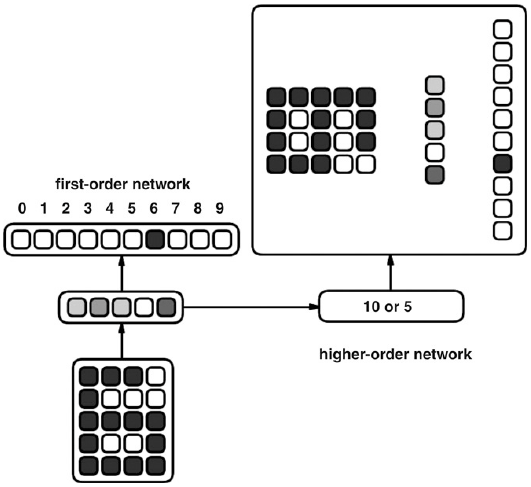
\includegraphics[width=240px]{../cleeremans_2007/digit_reco/digit_reco.png}
\end{center}
\caption{ \protect \footnotemark Architecture connexionniste avec méta-représentations  }
\end{figure}
\footnotetext{ Cleeremans, A., et al. Consciousness and 
metarepresentation : A computational sketch }

Nous avons réalisé que le second réseau\,\footnote{high-order network} apprenait 
plus vite sa tâche que le premier\,\footnote{first-order network}
uniquement parce que les entrées étaient faciles à reproduire. De plus, les entrées
étant plus nombreuses, elles ont un poids plus élevé dans la formule RMS. Ce qui 
explique le comportement des courbes de l'article.
\newline
Par ailleurs, nous avons remarqué que les neurones de la couche caché du premier
réseau se stabilisaient très rapidement ( autour de la 50\up{ième} époque ), le tout
permettant au second réseau d'avoir des entrées très peu variables, favorisant donc son
apprentissage.
\newline
Lorsque nous avons 
augmenté le nombre d'entrées en passant sur des chiffres manuscrits ( et en 
augmentant proportionnellement le nombre de neurones à l'intérieur des couches
cachés ), les performances du second réseau se sont écroulées : il n'était alors
plus que capable de reproduire la couche de sortie.
\newline
Enfin, nous avons remarqué qu'en bloquant l'apprentissage entre la couche cachée et les 
entrées du premier réseau, puis en changeant de tâche, le réseau était capable de réapprendre
la nouvelle tâche, ce qui prouve la présence d'une représentation des entrées dans la couche 
caché.
\newline
\newline
Il faut cependant remarquer qu'un simple perceptron est suffisant pour réaliser la tâche
du premier réseau, et donc, qu'il est possible que dans le cas d'un problème non linéairement
séparable cette architecture soit invalidé.

\section{Parier sur le premier réseau}

Rappelons également la structure des réseaux :
\begin{figure}[h]
\begin{center}
 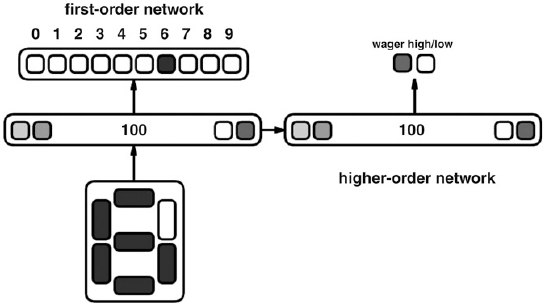
\includegraphics[width=280px]{../cleeremans_2007/digital_reco/schema.png}
\end{center}
 \caption{ \protect \footnotemark Architecture connexionniste avec paris  }
\end{figure}
\footnotetext{ Cleeremans, A., et al. Consciousness and 
metarepresentation : A computational sketch }

La première chose que nous avons faites à été d'améliorer les performances du second réseau
en modifiant quelques paramètres. Contrairement à celui de l'article, il ne se contentera 
plus simplement de parier haut à chaque coups ( après 40 époques). Il aura une longueur d'avance
sur le premier réseau sur toute la durée de l'apprentissage.

À partir de cette différence de performances, nous avons imaginer plusieurs architectures, qui
améliore plus ou moins les performances de reconnaissance du réseau sur des chiffres manuscrits:

\begin{figure}[h]
 \begin{center}
\begin{tabular}{c|c}
 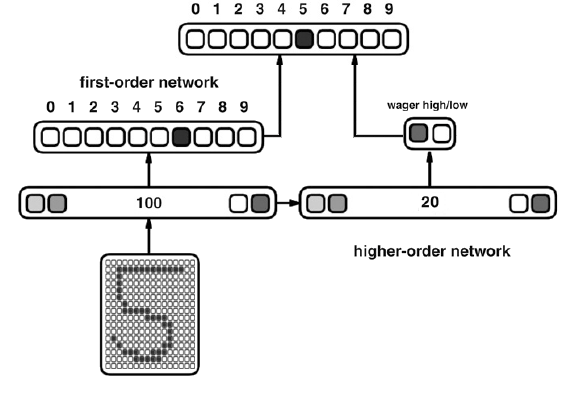
\includegraphics[width=210px]{../pre-presentation/thrid.png} & 
 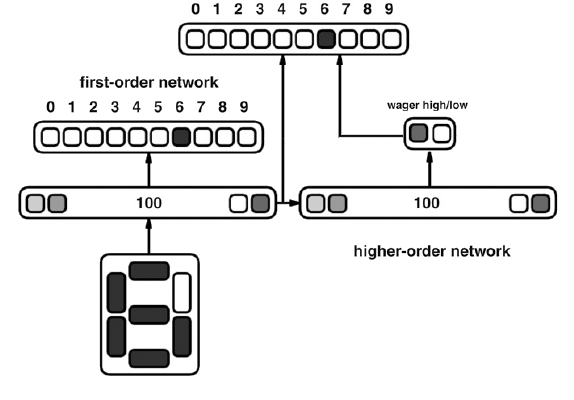
\includegraphics[width=210px]{../pre-presentation/thrid_hidden.png}
\end{tabular}
\end{center}
\caption{Architecture avec 3\up{ième} réseau}
\end{figure}

Dans ces 2 architectures, nous nous contentons de connecter un 3\up{ième} réseau qui doit 
tirer des conclusions à partir d'informations sur les 2 premiers.

\begin{figure}[h]
 \begin{center}
 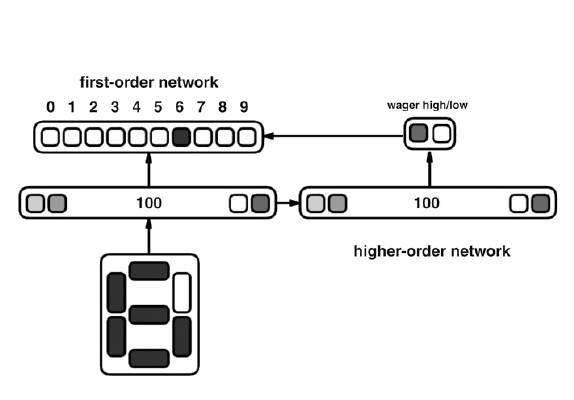
\includegraphics[width=250px]{../pre-presentation/merging.png}
\end{center}
\caption{Architecture par fusion}
\end{figure}

Ici, nous mélangeons un apprentissage par descente de gradient ( sur le premier et second réseau )
et un apprentissage perceptron ( entre les 2 couches de sorties ).

\begin{figure}[h]
 \begin{center}
 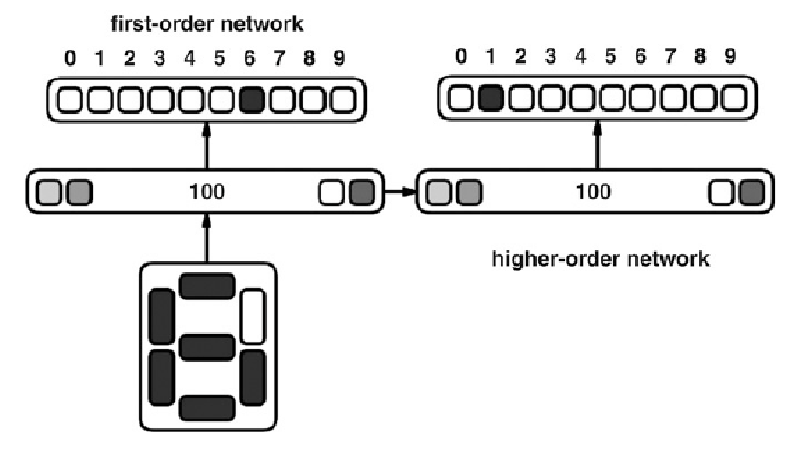
\includegraphics[width=300px]{../pre-presentation/nth_wta.png}
\end{center}
\caption{Architecture par intuitions}
\end{figure}

Cette architecture est légèrement différente dans le sens où elle n'enregistre
plus de pari mais l'indice du n\up{ième} neurone le plus actif contenant la bonne réponse.
Exemple : le réseau supérieur sort 2 -> la réponse est le 3\up{ième} neurone le plus actif 
de la couche de sortie du premier réseau.
\newline

Nous avons aussi essayer quelques modèles où le réseau supérieur servait de superviseur
à l'apprentissage du premier réseau. Par exemple, s'il pari haut, l'apprentissage du premier réseau
sera faible, sinon il sera accentué.

\section{La suite}

Ce que nous continuons d'étudier : 
\begin{itemize}
 \item validation sur des expériences plus complexes ( qui ne peuvent être résolue directement par un perceptron )
 \item relation entre la taille de la couche caché du premier réseau et le taux de paris avantageux
 \item de nouvelles architectures
\end{itemize}


\end{document}
